%%%%%%%%%%%%%%%%%%%%%%%%%%%%%%%%%%%%%%%%%
% NIWeek 2014 Poster by T. Reveyrand
% www.microwave.fr
% http://www.microwave.fr/LaTeX.html
% ---------------------------------------
%
% Original template created by:
% Brian Amberg (baposter@brian-amberg.de)
%
% This template has been downloaded from:
% http://www.LaTeXTemplates.com
%
% License:
% CC BY-NC-SA 3.0 (http://creativecommons.org/licenses/by-nc-sa/3.0/)
%
%%%%%%%%%%%%%%%%%%%%%%%%%%%%%%%%%%%%%%%%%

%----------------------------------------------------------------------------------------
%	PACKAGES AND OTHER DOCUMENT CONFIGURATIONS
%----------------------------------------------------------------------------------------

\documentclass[a0paper,portrait]{baposter}

\usepackage[T1]{fontenc}
\usepackage{mathtools, graphicx, xurl, hyperref}
% \usepackage{tikz-cd}
\usepackage{tikz}
\usetikzlibrary{shapes, arrows.meta, decorations.pathmorphing, decorations.pathreplacing, backgrounds, positioning, fit, calc, shadows, shapes.misc}
% \tikzexternalize[prefix=tikz/,optimize command away=\includepdf]
\usepackage{boldline, multirow}
\usepackage{booktabs} % Allows the use of \toprule, \midrule and \bottomrule in tables
\usepackage{colortbl}
\usepackage{subcaption}
\usepackage{relsize}
\usepackage{fontawesome5}
\usepackage[ruled, vlined]{algorithm2e}

\usepackage{tabularx} % for 'X' col. type and 'tabularx' environment
\usepackage{ragged2e} % for '\RaggedRight' macro
\newcolumntype{L}{>{\RaggedRight}X} % disable full justification

\usepackage{adjustbox}

% \tikzstyle{smallcircleblock} = [circle, draw, text width = 0.7em, text centered]

% \tikzstyle{wideblock} = [rectangle, draw, text width = 6.5em, text centered, rounded corners, inner sep = 7pt, minimum height = 1.0em]

\newcommand\ImageNode[4][]{
  \node[#1] (#2) {\includegraphics[#3]{#4}};
}
\definecolor{arrowblue}{RGB}{98,145,224}


\newcolumntype{g}{>{\columncolor[gray]{0.8}}l}


\newif\ifcoloredtext
\coloredtextfalse

\newif\ifboxednn
\boxednntrue


% --- unify spacing between floats and text (single-/double-column) ---
\setlength{\textfloatsep}{6pt plus 2pt minus 2pt}   % text <-> single-column floats (table/figure)
\setlength{\intextsep}{6pt plus 2pt minus 2pt}      % inline [h] floats
\setlength{\floatsep}{6pt plus 2pt minus 2pt}       % float <-> float (single-column)

\setlength{\dbltextfloatsep}{6pt plus 2pt minus 2pt} % text <-> double-column floats (figure*)
\setlength{\dblfloatsep}{6pt plus 2pt minus 2pt}     % float <-> float (double-column)

% --- caption spacing for tables only ---
\captionsetup[table]{aboveskip=6pt, belowskip=0pt}


\newenvironment{indentedquote}[1]%
{\list{}{\leftmargin=#1\rightmargin=#1}\item[]}%
{\endlist}


\newcommand\wordcount{\input{|"texcount -inc -sum -0 -utf8 -ch -template={SUM} \currfilepath"}}


\usepackage{textcomp}
\usepackage{eso-pic}
\usepackage{enumitem}
\usepackage{hyperref}

\setlist[itemize]{
  itemsep=1.5pt,
  topsep=3pt,
  parsep=0pt,
  partopsep=0pt,
  leftmargin=1em,
  labelsep=0.4em
}

\setlength{\abovedisplayskip}{3pt plus 1pt minus 1pt}
\setlength{\belowdisplayskip}{3pt plus 1pt minus 1pt}

\graphicspath{{images/}} % Directory in which figures are stored

\definecolor{bordercol}{RGB}{40,40,40} % Border color of content boxes
\definecolor{headercol1}{RGB}{186,215,230} % Background color for the header in the content boxes (left side)
\definecolor{headercol2}{RGB}{120,120,120} % Background color for the header in the content boxes (right side)
\definecolor{headerfontcol}{RGB}{0,0,0} % Text color for the header text in the content boxes
\definecolor{boxcolor}{RGB}{210,235,250} % Background color for the content in the content boxes

\definecolor{jdhblue}{RGB}{2,93,186}

\definecolor{zkblue}{RGB}{88,135,175}
\definecolor{zkbackground}{RGB}{230,232,234}


% \usetikzlibrary{shapes, arrows, external, decorations.pathmorphing, backgrounds, positioning, fit, petri, calc, hobby, cd}


\begin{document}

% \background{ % Set the background to an image (background.pdf)
% \begin{tikzpicture}[remember picture,overlay]
% \draw (current page.north west)+(-2em,2em) node[anchor=north west]
% {\includegraphics[height=1.1\textheight]{images/baposter_background.pdf}};
% \end{tikzpicture}
% }

% add conference banner
\AddToShipoutPictureFG*{%
  \AtPageLowerLeft{%
    \hspace{0.82em}
    \raisebox{0.2ex}{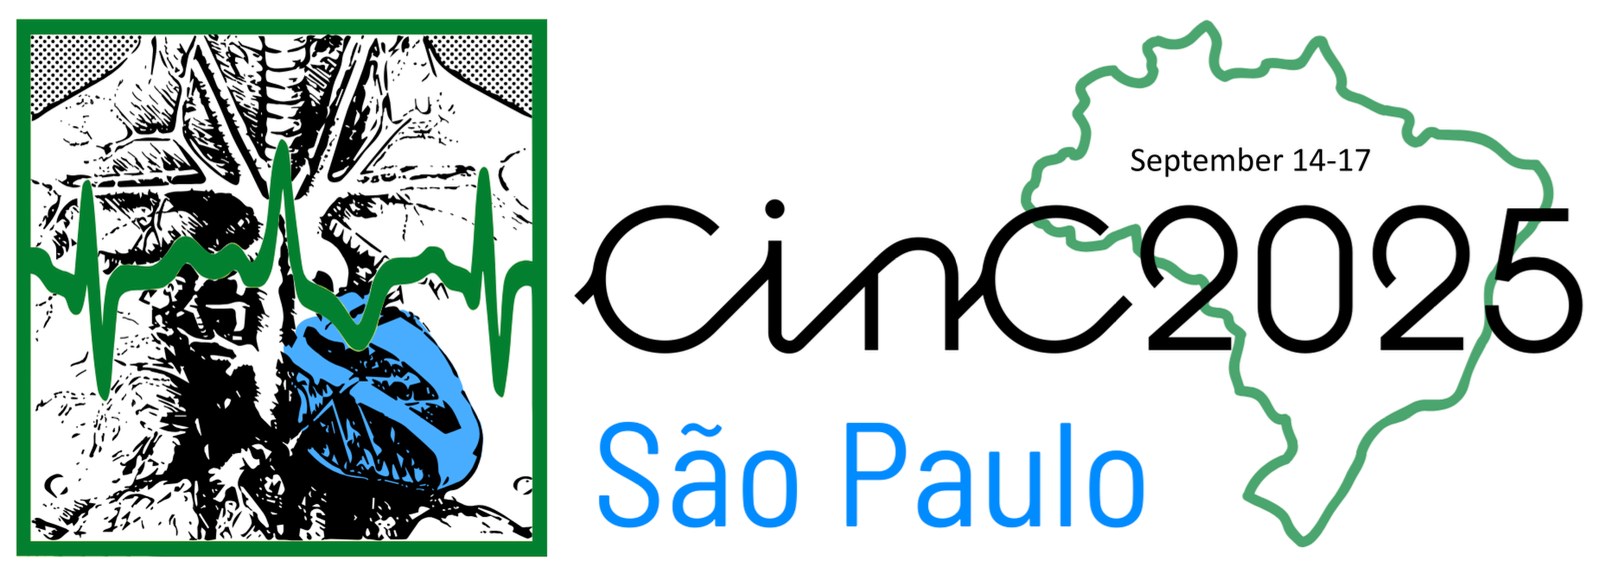
\includegraphics[width=0.16\textwidth]{cinc2025-banner.png}}
  }
}

\begin{poster}{
grid=false,
borderColor=bordercol, % Border color of content boxes
headerColorOne=headercol1, % Background color for the header in the content boxes (left side)
headerColorTwo=headercol2, % Background color for the header in the content boxes (right side)
headerFontColor=headerfontcol, % Text color for the header text in the content boxes
% boxColorOne=boxcolor, % Background color for the content in the content boxes
boxColorOne=zkbackground,
headershape=roundedright, % Specify the rounded corner in the content box headers
headerfont=\Large\sf\bf, % Font modifiers for the text in the content box headers
textborder=rectangle,
% background=user,
background=none,
headerborder=open, % Change to closed for a line under the content box headers
boxshade=plain
}
%
%----------------------------------------------------------------------------------------
%	TITLE AND AUTHOR NAME
%----------------------------------------------------------------------------------------
%
{
\includegraphics[scale=0.401]{logo_cau_science.png}} % University/lab logo
{
{\bf \fontsize{19pt}{19pt} \selectfont Reliability-Aware Hierarchical Learning for Chagas Detection from ECG under Expert Label Scarcity}
} % Poster title
{\vspace{0.3em} \smaller Hao WEN$^1$, Jingsu KANG$^2$  \\  % Author names

$^1${\it College of Science, China Agricultural University}\qquad
$^2${\it Tianjin Medical University} \\
\vspace{0.2cm}
{\Large \bf{The George B. Moody PhysioNet Challenge 2025}, ~~~\bf{Team Revenger}}
}
{
\includegraphics[scale=0.101]{logo_tmu.jpeg}}


\newif\ifcoloredtext
\coloredtexttrue
\newif\ifboxednn
\boxednntrue


%----------------------------------------------------------------------------------------
%	INTRODUCTION & CHALLENGE CONTEXT
%----------------------------------------------------------------------------------------

\headerbox{Proposed Reliability-Aware Framework}{name=introduction, column=0, row=0, span=3}{

\begin{itemize}
\item {\bf Team Revenger – PhysioNet Challenge 2025}: ECG-based Chagas cardiomyopathy screening in resource-limited settings
\item {\bf Challenge objective}: Maximize positive case retrieval under 5\% prevalence constraint for scalable screening
\item {\bf Key challenge}: Severe class imbalance ($\sim$2\% positives) + expert label scarcity (0.2\% expert-confirmed)
\item {\bf Our approach}: Reliability-aware hierarchical learning prioritizing expert-confirmed over self-reported labels
\end{itemize}

}

%----------------------------------------------------------------------------------------
%	DATA & LABEL PROVENANCE
%----------------------------------------------------------------------------------------

\headerbox{Data \& Label Provenance}{name=data, column=0, row=1, span=2, below=introduction}{

Three ECG datasets with heterogeneous label reliability and Chagas prevalence:

\begin{center}
\begin{tabular}{rlll}
\toprule
Dataset & \multicolumn{1}{c}{N} & \multicolumn{1}{c}{Chagas \%} & Label source \\
\midrule
SaMi-Trop   & 1,631     & 100.0 \%    & expert-confirmed \\
CODE-15\%   & 345,779   & 1.8 \%      & self-reported \\
PTB-XL      & 21,799    & 0.0 \%      & N/A (non-endemic) \\
\bottomrule
\end{tabular}
\end{center}

\begin{itemize}
\item {\bf Preprocessing}: Resampled to 400 Hz, bandpass filtered (0.5–45 Hz), z-score normalized
\item {\bf Challenge}: Model must learn from heterogeneous label quality and extreme class imbalance
\end{itemize}

}

%----------------------------------------------------------------------------------------
%	RELIABILITY-AWARE SUPERVISION
%----------------------------------------------------------------------------------------

\headerbox{Reliability-Aware Supervision}{name=supervision, column=2, row=1, span=1, below=introduction}{

{\bf Label Smoothing \& Upsampling Strategy}

Hierarchical supervision encoding source reliability through stratified label smoothing:
\[
\text{\bf Formula:} ~~ \tilde{\mathbf{y}} = (1 - \varepsilon) \cdot \mathbf{y} + \frac{\varepsilon}{C} \cdot \mathbf{1}
\]
Where smoothing factor $\varepsilon$ depends on reliability:
\begin{itemize}
\item SaMi positives: $\varepsilon = 0.0$ (max trust)
\item CODE-15\% samples: $\varepsilon = 0.6$ (uncertainty)  
\item PTB-XL negatives: $\varepsilon = 0.2$ (mild regularization)
\end{itemize}

\vspace{0.3cm}
\begin{center}
\begin{tabular}{ccc}
\toprule
\multicolumn{2}{c}{Upsample factor} & \multirow{2}{*}{Score} \\
\cmidrule(lr){1-2}
CODE & SaMi & \\
\midrule
3 & 12    & \textbf{0.245} \\
3 & 7     & 0.212 \\
10 & 120   & 0.210 \\
\bottomrule
\end{tabular}
\end{center}

}

%----------------------------------------------------------------------------------------
%	MODEL ARCHITECTURE
%----------------------------------------------------------------------------------------

\headerbox{Model Architecture}{name=architecture, column=0, row=2, span=1, below=data}{

{\bf Enhanced 1D ResNet with SE Modules}

\begin{center}
\resizebox{1.03\linewidth}{!}{%
  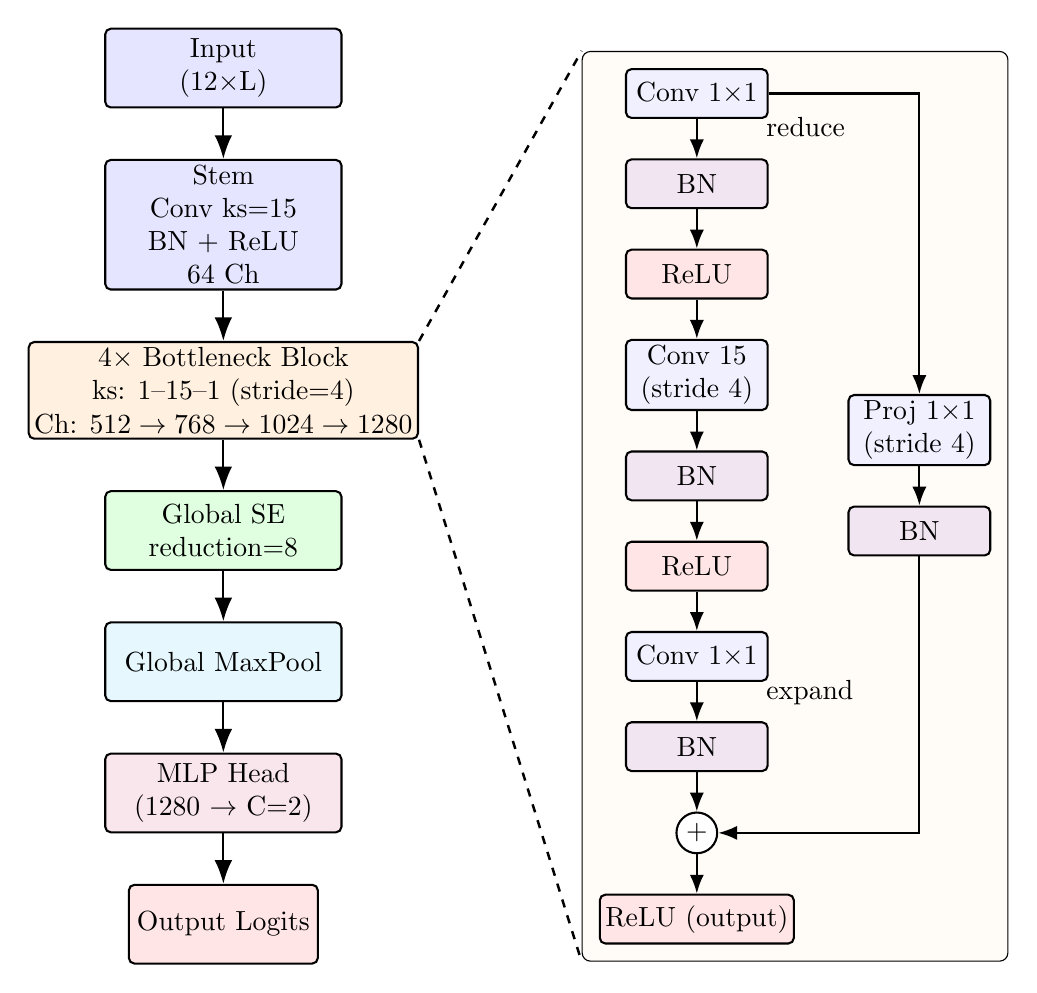
\begin{tikzpicture}[
    % font=\small,
    line width=0.75pt,
    >={Latex[length=3mm]},
    node distance=6.4mm,
    every node/.style={inner sep=2pt},
    stem/.style={draw, rounded corners=2pt, minimum width=30mm, minimum height=10mm,
                 align=center, fill=blue!10},
    block/.style={draw, rounded corners=2pt, minimum width=30mm, minimum height=12mm,
                  align=center, fill=orange!12},
    se/.style={draw, rounded corners=2pt, minimum width=30mm, minimum height=10mm,
               align=center, fill=green!12},
    pool/.style={draw, rounded corners=2pt, minimum width=30mm, minimum height=10mm,
                 align=center, fill=cyan!10},
    head/.style={draw, rounded corners=2pt, minimum width=30mm, minimum height=10mm,
                 align=center, fill=purple!10},
    output/.style={draw, rounded corners=2pt, minimum width=24mm, minimum height=10mm,
                align=center, fill=red!10},
    arrow/.style={-{Latex[length=3mm]}, thick},
    darr/.style={-{Latex[length=2.4mm]}, thick},
    dashedarrow/.style={-{Latex[length=2.6mm]}, thick, dashed},
    ann/.style={inner sep=1pt, align=center},
    layer/.style={draw, rounded corners=2pt, minimum width=18mm, minimum height=6.2mm,
                  align=center, fill=blue!6},
    bnact/.style={draw, rounded corners=2pt, minimum width=18mm, minimum height=6.2mm,
                  align=center, fill=violet!10},
    act/.style={draw, rounded corners=2pt, minimum width=18mm, minimum height=6.2mm,
                  align=center, fill=red!10},
    drop/.style={draw, rounded corners=2pt, minimum width=18mm, minimum height=6.2mm,
                  align=center, fill=gray!15, dashed},
    sum/.style={draw, circle, inner sep=1.6pt, fill=white},
    % brace/.style={decorate, decoration={brace, amplitude=6pt}},
    detailbox/.style={draw, rounded corners=3pt, inner sep=6pt, fill=orange!3}
]

% ================= Left (overall vertical path) =================
\node[stem] (input) {Input \\ (12$\times$L)};
\node[stem, below=of input] (stem) {Stem \\ Conv ks=15 \\ BN + ReLU \\ 64 Ch};

% Compressed single bottleneck block (represents 4 stacked blocks)
\node[block, below=of stem] (bottleneck) {$4 \times$ Bottleneck Block \\ ks: 1--15--1 (stride=4) \\ Ch: $512 \to 768 \to 1024 \to 1280$};

% Global SE
\node[se, below=of bottleneck] (gse) {Global SE \\ reduction=8};

% Global pooling
\node[pool, below=of gse] (gap) {Global MaxPool};

% MLP Head
\node[head, below=of gap] (mlp) {MLP Head \\ (1280 $\rightarrow$ C=2)};

% Output
\node[output, below=of mlp] (out) {Output Logits};

% Arrows (overall path)
\draw[arrow] (input) -- (stem);
\draw[arrow] (stem) -- (bottleneck);
\draw[arrow] (bottleneck) -- (gse);
\draw[arrow] (gse) -- (gap);
\draw[arrow] (gap) -- (mlp);
\draw[arrow] (mlp) -- (out);

% ================= Right (expanded single bottleneck internals) =================
% Anchor for expansion (to the right of overall bottleneck block)
\coordinate (expandAnchor) at ($(input.east)+(45mm,0)$);

\node[layer, below=0mm of expandAnchor] (c1) {Conv 1$\times$1};
\node[below right=-1mm and 8mm of c1.south] {reduce};
\node[bnact, below=5mm of c1] (bn1) {BN};
\node[act, below=5mm of bn1] (a1) {ReLU};

\node[layer, below=5mm of a1] (c2) {Conv 15\\(stride 4)};
\node[bnact, below=5mm of c2] (bn2) {BN};
\node[act, below=5mm of bn2] (a2) {ReLU};
% \node[drop, below=5mm of a2] (drp) {Dropout 0.2};

\node[layer, below=5mm of a2] (c3) {Conv 1$\times$1};
\node[below right=-1mm and 8mm of c3.south] {expand};
\node[bnact, below=5mm of c3] (bn3) {BN};

\node[sum, below=5mm of bn3] (add) {+};
\node[act, below=5mm of add] (outact) {ReLU (output)};

% Projection/skip branch (since stride=4 or channel change)
\node[layer, right=10mm of c2, yshift=-7mm, minimum width=18mm] (proj) {Proj 1$\times$1 \\ (stride 4)};
\node[bnact, below=5mm of proj, minimum width=18mm] (projbn) {BN};

% Connections internal
\draw[darr] (c1) -- (bn1);
\draw[darr] (bn1) -- (a1);
\draw[darr] (a1) -- (c2);
\draw[darr] (c2) -- (bn2);
\draw[darr] (bn2) -- (a2);
% \draw[darr] (a2) -- (drp);
\draw[darr] (a2) -- (c3);
\draw[darr] (c3) -- (bn3);
\draw[darr] (bn3) -- (add);
\draw[darr] (add) -- (outact);

% Skip path
\draw[darr] (c1.east) -| ($(proj.north)+(0,0mm)$);
\draw[darr] (proj) -- (projbn);
\draw[darr] (projbn.south) |- (add.east);

\begin{scope}[on background layer]
\node[detailbox, fit=(c1) (bn1) (a1) (c2) (bn2) (a2) (c3) (bn3) (proj) (projbn) (add) (outact)] (detail) {};
\end{scope}

\draw[dashed, line width=0.9pt] (bottleneck.north east) -- (detail.north west);
\draw[dashed, line width=0.9pt] (bottleneck.south east) -- (detail.south west);

\end{tikzpicture}

}
\end{center}

\begin{itemize}
\item {\bf Bottleneck blocks}: 1-15-1 convolutions, expansion factor 4, stride 4 downsampling
\item {\bf Global SE}: Channel attention, reduction ratio 8 for temporal feature recalibration  
\item {\bf Variable-length inputs}: Global MaxPool enables inference on ECGs of any duration
\end{itemize}

}

%----------------------------------------------------------------------------------------
%	TRAINING & OPTIMIZATION
%----------------------------------------------------------------------------------------

\headerbox{Training \& Optimization}{name=training, column=1, row=2, span=1, below=data}{

% {\bf Asymmetric Loss \& Optimization Setup}

\begin{itemize}
\item {\bf Asymmetric Loss}: $L = -y(1-p)^{\gamma_{+}} \log(p) - (1-y)(p_m)^{\gamma_{-}} \log(1-p_m)$
\item Parameters: $(\gamma_{+},\gamma_{-})=(1,4)$, margin $\delta=0.05$
\item {\bf Optimizer}: AdamW
\item {\bf LR Scheduler}: OneCycle
\item {\bf LR}: $1 \times 10^{-4}$ initial, $6 \times 10^{-4}$ peak
\item {\bf Training}: 30 epochs, batch size 128, weight decay $1 \times 10^{-2}$
\item {\bf Input}: 4,096 samples (uniform crop/center trim)
\item {\bf Early stopping}: Challenge score on 20\% internal hold-out subset
\end{itemize}

}

%----------------------------------------------------------------------------------------
%	RESULTS
%----------------------------------------------------------------------------------------

\headerbox{Results}{name=results, column=0, row=3, span=3, below=architecture}{

{\bf Challenge Performance \& Analysis}

\begin{center}
\begin{tabular}{r|r|r|r}
Internal hold-out (mean±std) & Hidden validation & Rank & Test \\
\hline
$0.451 \pm 0.005$ & 0.245 & 179/364 & TBA \\
\hline
\end{tabular}
\end{center}

\begin{itemize}
\item {\bf Hidden validation score}: 0.245 (Challenge metric: TPR at 5\% prevalence constraint)
\item {\bf Performance gap}: Internal vs. hidden suggests domain shift or overfitting to public data
\item {\bf Key insight}: Reliability-aware supervision stabilizes learning under noisy labels more effectively than architectural complexity alone
\end{itemize}

}

%----------------------------------------------------------------------------------------
%	DISCUSSION & INSIGHTS
%----------------------------------------------------------------------------------------

\headerbox{Discussion \& Insights}{name=discussion, column=0, row=4, span=2, below=results}{

{\bf How does the approach provide insight into the Challenge issues?}

\begin{itemize}
\item {\bf Label provenance modeling}: Explicitly encoding expert vs. self-reported reliability addresses core challenge of heterogeneous label quality in multi-source ECG datasets
\item {\bf Hierarchical supervision}: Dynamic smoothing factors prevent overconfident gradients on noisy labels while preserving sharp supervision on expert-confirmed cases
\item {\bf Scalability}: Framework aligns with clinical reality—expert labels are scarce but high-quality; self-reported labels are abundant but uncertain
\item {\bf Performance gap analysis}: Static reliability weights may not capture within-source label heterogeneity; adaptive weighting could improve generalization
\end{itemize}

}

%----------------------------------------------------------------------------------------
%	FUTURE WORK
%----------------------------------------------------------------------------------------

\headerbox{Future Work}{name=future, column=2, row=4, span=1, below=results}{

{\bf Adaptive Supervision Framework}

\begin{itemize}
\item {\bf Dynamic reliability}: Learn instance-specific confidence scores vs. static smoothing factors
\item {\bf Adaptive sampling}: Confidence-aware upsampling responding to model evolution during training
\item {\bf Data augmentation}: CutMix, SMOTE for positive sample diversification
\item {\bf Multi-task learning}: Leverage auxiliary arrhythmia labels for enhanced feature representation
\item {\bf Self-supervised pre-training}: Large-scale unlabeled ECG data for transferable representations
\end{itemize}

}

%----------------------------------------------------------------------------------------
%	ACKNOWLEDGEMENTS
%----------------------------------------------------------------------------------------

% \headerbox{Acknowledgements}{name=acknowledgements, column=0, row=5, span=3, below=discussion}{

% We thank Professor {\bf Deren Han} from the School of Mathematical Sciences, Beihang University for providing GPU servers. We acknowledge the PhysioNet Challenge organizers and the contributing datasets.

% }

%----------------------------------------------------------------------------------------
%	REFERENCES
%----------------------------------------------------------------------------------------

% \headerbox{References}{name=references, column=0, row=6, span=3, below=acknowledgements}{

% \begin{thebibliography}{9}
% \bibitem{goldberger2000} Goldberger AL, et al. PhysioBank, PhysioToolkit, and PhysioNet. {\it Circulation} 2000;101(23):e215-e220.
% \bibitem{ribeiro2020} Ribeiro AH, et al. Automatic diagnosis of the 12-lead ECG using a deep neural network. {\it Nat Commun} 2020;11:1760.
% \bibitem{hu2018} Hu J, et al. Squeeze-and-Excitation Networks. {\it CVPR} 2018:7132-7141.
% \bibitem{ridnik2021} Ridnik T, et al. Asymmetric Loss For Multi-Label Classification. {\it ICCV} 2021:82-91.
% \bibitem{yun2019} Yun S, et al. CutMix: Regularization Strategy to Train Strong Classifiers. {\it ICCV} 2019:6023-6032.
% \bibitem{chawla2002} Chawla NV, et al. SMOTE: Synthetic Minority Oversampling Technique. {\it JAIR} 2002;16:321-357.
% \end{thebibliography}

% }

%----------------------------------------------------------------------------------------
%	FOOTER
%----------------------------------------------------------------------------------------

\headerbox{}{name=foottext, column=0, span=3, below=future, textborder=none, headerborder=none, boxheaderheight=0pt}{
\hfill \small \textit{Code, configs, etc. are available at https://github.com/wenh06/cinc2025, and is based on https://github.com/DeepPSP/torch\_ecg.}
}

\end{poster}

\end{document}
